\documentclass[conference]{IEEEtran}
\usepackage[utf8]{inputenc}
\usepackage[portuguese]{babel}
\usepackage{amsmath,amssymb,amsfonts}
\usepackage{algorithm}
\usepackage{algorithmic}
\usepackage{graphicx}
\usepackage{textcomp}
\usepackage{xcolor}
\usepackage{booktabs}
\usepackage[caption=false,font=footnotesize]{subfig}
\usepackage{stfloats}
\usepackage{pgfplots}
\pgfplotsset{compat=1.17}
\usepackage{url}
\usepackage{cite}
\usepackage{listings}

\lstset{
    language=Python,
    basicstyle=\ttfamily\footnotesize,
    keywordstyle=\color{blue},
    stringstyle=\color{red},
    commentstyle=\color{gray},
    numbers=left,
    numberstyle=\tiny\color{gray},
    stepnumber=1,
    breaklines=true,
    frame=single,
    showstringspaces=false
}

\begin{document}
\title{Sistema Híbrido de Recomendação em Grafos Bipartidos: Mitigando o Viés de Popularidade e a Ambiguidade Taxonômica na Plataforma Steam}

\author{
    \IEEEauthorblockN{Gabriel Alves Faria\IEEEauthorrefmark{1}, Rafael Alves Faria\IEEEauthorrefmark{1}, Michel Pires da Silva\IEEEauthorrefmark{2}}
    \IEEEauthorblockA{\IEEEauthorrefmark{1}Departamento de Computação -- Centro Federal de Educação Tecnológica de Minas Gerais (CEFET-MG)\\
    Campus V -- Divinópolis, MG, Brasil\\
    Email: gabrielalvesfaria@gmail.com, rafael16alvesf@gmail.com}
    \IEEEauthorblockA{\IEEEauthorrefmark{2}Orientador -- CEFET-MG / UFCI-MG\\
    Divinópolis, MG, Brasil\\
    Email: michel@cefetmg.br}
}

\maketitle

% ==============================================================================
% RESUMO / ABSTRACT (Máximo 250 palavras, respondendo diretamente às 4 perguntas da Seção 3.2 de pratica.pdf)
% 1. Qual o problema?
% 2. Há soluções, quais?
% 3. Como foi modelado (qual estrutura)?
% 4. Qual o principal resultado obtido?
% ==============================================================================
\begin{abstract}
A proliferação exponencial dos catálogos de jogos digitais impõe severos desafios aos Sistemas de Recomendação convencionais, que frequentemente falham devido ao viés de popularidade de \textit{super-hubs} virais em abordagens colaborativas e à ambiguidade de macrocategorias burocráticas genéricas (como Ação e Aventura) na filtragem por conteúdo. Modelos baseados em redes neurais profundas tentam contornar essas limitações, contudo demandam alto custo computacional e carecem de interpretabilidade estrutural. Este trabalho propõe uma arquitetura híbrida fundamentada em teoria dos grafos e estruturas de dados em memória principal. O ecossistema de consumo da plataforma Steam é modelado como um grafo bipartido ponderado usuário--jogo submetido a uma poda adaptativa $K$-Core orientada pela mediana de tempo de jogo (piso de 5,0 horas) e poda prévia de qualidade ($positive\_ratio \ge 65\%$). A macroestrutura da rede é particionada em comunidades modulares via Algoritmo de Louvain determinístico, enquanto a recuperação de candidatos é executada por uma Busca em Largura (BFS) em dois níveis suportada por estruturas de dispersão com tempo de acesso amortizado $O(1)$. O ranqueamento final integra similaridade contínua de Ruzicka com $\text{IDF}^2$ ponderado por consenso comunitário, filtros de dissonância de tom, desempate por categorias oficiais, prior bayesiano de qualidade e amortecimento topológico de grau de \textit{super-hubs}. A validação experimental via protocolo \textit{Leave-One-Out} em 300 usuários demonstrou ganho de até 77,3\% em Hit Rate@10 frente ao modelo sem amortecimento e alta precisão na segregação de subnichos mecânicos com tempo de resposta inferior a 200 milissegundos em CPU comum.
\end{abstract}

\begin{IEEEkeywords}
Sistemas de Recomendação, Grafos Bipartidos, Detecção de Comunidades, Algoritmo de Louvain, Tabelas de Dispersão, TF-IDF, Plataforma Steam.
\end{IEEEkeywords}

% ==============================================================================
% SEÇÃO I: INTRODUÇÃO
% ==============================================================================
\section{Introdução}

A indústria global de jogos eletrônicos consolidou-se como um dos setores de maior faturamento na economia contemporânea do entretenimento, impulsionada pela ampla adesão à distribuição digital em plataformas como a \textit{Steam}. Todavia, a disponibilização contínua de dezenas de milhares de títulos gera um fenômeno conhecido na literatura como sobrecarga informacional (\textit{information overload}), desencadeando o "Paradoxo da Escolha", no qual a abundância excessiva de opções, desprovida de mecanismos eficazes de triagem, induz à paralisia decisória e à insatisfação do consumidor. Nesse cenário, os Sistemas de Recomendação (\textit{Recommender Systems} --- RecSys) tornaram-se componentes essenciais de infraestrutura para a descoberta de conteúdo e sustentabilidade dos catálogos.

Entretanto, a recomendação de jogos eletrônicos apresenta peculiaridades intrínsecas que desafiam os algoritmos clássicos concebidos para comércio eletrônico ou streaming de mídia:
\begin{enumerate}
    \item \textbf{Heterogeneidade do Engajamento Temporal}: Diferente da duração padronizada de uma produção audiovisual, o tempo de jogo varia em ordens de magnitude. Quinze horas de jogabilidade representam a conclusão integral de uma obra narrativa de campanha linear curta, mas configuram apenas um contato preliminar ou casual em simuladores, mundos abertos ou títulos cooperativos.
    \item \textbf{Viés de Popularidade e Super-Hubs}: Abordagens de filtragem puramente colaborativas (\textit{Collaborative Filtering} --- CF) sofrem com a proliferação de títulos gratuitos ou de apelo massivo (\textit{Counter-Strike}, \textit{Garry's Mod}, \textit{Left 4 Dead 2}) que atuam como "super-hubs", acumulando arestas de forma desproporcional e monopolizando as recomendações em detrimento de produções de nicho.
    \item \textbf{Ambiguidade e Diluição Taxonômica}: Sistemas estritamente baseados em conteúdo (\textit{Content-Based Filtering} --- CBF) dependem de metadados fornecidos pelas publicadoras, que recorrentemente atribuem categorias burocráticas genéricas (como \textit{Action} e \textit{Adventure}) a mais de 80\% das obras, gerando falsas equivalências entre jogos com mecânicas diametralmente opostas (como quebra-cabeças infantis e títulos de sobrevivência pós-apocalípticos).
\end{enumerate}

Trabalhos precursores desenvolvidos no próprio CEFET-MG (Campus Divinópolis), como o sistema híbrido de recomendação de filmes proposto por Amorim Neto \cite{amorim2024}, evidenciaram que a combinação de modelagens em grafos com o particionamento comunitário de Louvain é altamente eficaz para capturar agrupamentos orgânicos de interesse. Contudo, a aplicação dessa estratégia ao domínio de jogos exige superar desafios específicos de engajamento temporal assimétrico e contaminação semântica por termos superficiais.

Diante dessa problemática, a motivação deste trabalho reside na concepção de um sistema híbrido de recomendação que explore a topologia estrutural de redes complexas em conjunto com a semântica fina de tags atribuídas pela comunidade de jogadores, sem recorrer a modelos neurais opacos que demandam treinamento custoso em aceleradores gráficos. A hipótese central investigada é que o casamento entre agrupamentos topológicos modulares e uma formulação contínua não-linear de pesos semânticos permite isolar comunidades genuínas de consumo e neutralizar a força bruta de nós onipresentes.

Os objetivos fundamentais desta pesquisa são:
\begin{enumerate}
    \item Modelar as interações de consumo da Steam como um grafo bipartido ponderado, aplicando uma estratégia de poda adaptativa $K$-Core orientada pela mediana móvel de horas (piso de 5,0 horas) e poda prévia de qualidade ($positive\_ratio \ge 65\%$);
    \item Identificar a macroestrutura do catálogo por meio de detecção de comunidades com o Algoritmo de Louvain, mapeando macro-clusters semânticos com reprodutibilidade determinística;
    \item Implementar um motor de busca em largura (BFS) em dois níveis suportado por indexação e memoização em tabelas de dispersão em memória principal com complexidade amortizada $O(1)$;
    \item Formular uma métrica contínua de similaridade de conteúdo baseada no Índice de Ruzicka com $\text{IDF}^2$ sobre tags comunitárias atenuadas por consenso, descarte por dissonância de tom, prior de qualidade e amortecimento topológico de grau de \textit{super-hubs};
    \item Validar experimentalmente a solução por meio de avaliações quantitativas (\textit{Leave-One-Out}, Hit Rate@10, NDCG@10 e análises de sensibilidade) e qualitativas em 104 títulos de referência, disponibilizando código aberto no GitHub \cite{github}, base tratada no Zenodo \cite{zenodo}, interface web interativa em produção no Render \cite{render} e exportações estruturadas para o Gephi inspiradas na clássica Figura 2 de Blondel \textit{et al.} \cite{blondel2008}.
\end{enumerate}

O restante deste artigo está organizado da seguinte forma: a Seção II apresenta o referencial teórico e os fundamentos de grafos e sistemas de recomendação. A Seção III detalha a metodologia proposta, descrevendo o tratamento de dados, a modelagem matemática, o ciclo de vida da aplicação e o algoritmo de ranqueamento. A Seção IV expõe e discute criticamente os resultados quantitativos, qualitativos, a visualização no Gephi e a eficiência computacional. Por fim, a Seção V apresenta as considerações finais, limitações e propostas de trabalhos futuros.

% ==============================================================================
% SEÇÃO II: REFERENCIAL TEÓRICO
% ==============================================================================
\section{Referencial Teórico}

\subsection{Modelagem em Grafos Bipartidos e Predição em Dois Saltos}
Conforme formalizado por Maier e Simovici \cite{maier2022}, relacionamentos de consumo do mundo real entre duas classes disjuntas de entidades são naturalmente mapeados como grafos bipartidos $G = (U \cup V, E)$, onde $U$ representa o conjunto de usuários, $V$ o conjunto de itens (jogos) e as arestas $e = (u, v) \in E$ denotam interações explícitas ou implícitas entre eles. Em sistemas de recomendação em grafos, a inferência de novos itens de interesse baseia-se na navegação de caminhos de comprimento 2 (2-\textit{hop paths}): parte-se de um vértice-alvo $v \in V$, resgatam-se os vizinhos adjacentes $u \in U$ com maior peso de afinidade e, a partir destes, expandem-se os itens candidatos $v' \in V$. Maier e Simovici ressaltam que grafos de recomendação em larga escala enfrentam severos desafios de esparsidade de dados (\textit{data sparsity}) e o problema de partida a frio (\textit{cold-start}), no qual novos nós sem conectividade prévia não podem ser alcançados puramente pela topologia da rede.

\subsection{Decomposição K-Core em Redes Complexas}
A decomposição $K$-Core, formalizada por Batagelj e Zaversnik \cite{batagelj2003}, é uma técnica de filtragem recursiva que extrai o subgrafo maximal induzido $H \subseteq G$ no qual todos os vértices possuem grau pelo menos $k$:
\begin{equation}
\forall v \in V(H), \quad \text{grau}_H(v) \ge k
\end{equation}
Em redes bipartidas usuário--item, adota-se um $K$-Core assimétrico $(k_U, k_V)$, exigindo que usuários possuam grau mínimo $k_U$ e itens grau mínimo $k_V$. Por ser uma propriedade recursiva, a eliminação de nós periféricos diminui o grau de seus vizinhos, exigindo iterações sucessivas até a estabilização matemática completa.

\subsection{Taxonomia de Sistemas de Recomendação}
No levantamento abrangente conduzido por Nagarnaik e Thomas \cite{nagarnaik2015}, as técnicas de recomendação são categorizadas em três paradigmas centrais:
\begin{itemize}
    \item \textbf{Filtragem Baseada em Conteúdo (CBF):} Avalia descritores intrínsecos dos itens para sugerir produtos semelhantes àqueles previamente consumidos. Embora imune à esparsidade de interações entre usuários, tende à superespecialização e não propicia descobertas fortuitas (\textit{serendipity});
    \item \textbf{Filtragem Colaborativa (CF):} Subdividida em abordagens baseadas em memória (\textit{memory-based}) e em modelos (\textit{model-based}). Métodos puramente baseados em memória sofrem de problemas crônicos de escalabilidade ($O(|U| \cdot |V|)$) e viés de popularidade;
    \item \textbf{Sistemas Híbridos:} Combinam a força preditiva do comportamento coletivo com os atributos semânticos de conteúdo. Nagarnaik e Thomas \cite{nagarnaik2015}, assim como Amorim Neto \cite{amorim2024}, enfatizam que a hibridização é a estratégia mais eficaz para mitigar as limitações individuais de esparsidade, escalabilidade e ambiguidade taxonômica.
\end{itemize}

\subsection{Detecção de Comunidades Modulares (Algoritmo de Louvain)}
Para dotar o grafo de uma representação em macroescala (\textit{model-based}), utiliza-se o Algoritmo de Louvain proposto por Blondel \textit{et al.} \cite{blondel2008}. O algoritmo é um método heurístico guloso que busca maximizar a métrica de modularidade $Q$, definida por:
\begin{equation}
Q = \frac{1}{2m} \sum_{i,j} \left[ A_{ij} - \frac{k_i k_j}{2m} \right] \delta(c_i, c_j)
\label{eq:louvain}
\end{equation}
onde $A_{ij}$ representa o peso da aresta entre os vértices $i$ e $j$, $k_i$ é a soma dos pesos das arestas conectadas ao vértice $i$, $m = \frac{1}{2}\sum_{ij} A_{ij}$, e $\delta(c_i, c_j)$ é a função delta de Kronecker que retorna 1 caso os vértices pertençam à mesma comunidade $c$, e 0 caso contrário. A identificação de comunidades permite atribuir um bônus de coesão topológica entre nós que compartilham o mesmo "super-nó".

\subsection{Tabelas de Dispersão e Estruturas de Pertinência em Memória}
A execução de buscas em largura em redes com milhões de arestas exige estruturas de dados de alta eficiência para controle de nós visitados e cálculo de funções de custo. Conforme fundamentado por Cormen \textit{et al.} \cite{cormen2009}, tabelas de dispersão (\textit{hash tables}) e conjuntos indexados fornecem operações fundamentais de inserção, remoção e consulta em tempo computacional médio $O(1)$. 

Embora filtros probabilísticos compactos como o Filtro de Bloom \cite{bloom1970} ofereçam alta economia espacial para testes de pertinência às custas de uma taxa controlada de falsos positivos, o presente trabalho emprega tabelas de dispersão convencionais em memória principal \cite{cormen2009}. Essa escolha garante determinismo temporal estrito, ausência absoluta de falsos positivos no descarte de arestas e memoização exata das similaridades semânticas contínuas entre pares de jogos durante a travessia da BFS, operando com consumo de memória estritamente proporcional à esparsidade da rede ($O(|V| + |E|)$).

\subsection{Ponderação Estatística de Termos (TF-IDF) e Índice de Ruzicka}
O modelo TF-IDF (\textit{Term Frequency-Inverse Document Frequency}) \cite{salton1988} avalia a importância relativa de um termo $t$ dentro de uma coleção de documentos $D$. A frequência inversa do documento é dada por:
\begin{equation}
\text{IDF}(t) = \ln\left(\frac{1 + |D|}{1 + df(t)}\right) + 1{,}0
\label{eq:idf}
\end{equation}
onde $|D|$ é a cardinalidade total do catálogo de jogos e $df(t)$ é a quantidade de títulos associados à tag $t$. Termos genéricos e onipresentes na plataforma (como \textit{Singleplayer} ou \textit{Action}) recebem valores de $\text{IDF}$ próximos a 1,0, enquanto tags descritoras de mecânicas de nicho (como \textit{Metroidvania} ou \textit{Souls-like}) obtêm valores substancialmente maiores. 

Para integrar esses pesos estatísticos de forma contínua, o Índice de Ruzicka (Jaccard Generalizado) opera sobre vetores ponderados calculando a razão entre a soma dos mínimos e a soma dos máximos das componentes, permitindo que variações contínuas de importância semântica modulem diretamente a afinidade entre itens.

% ==============================================================================
% SEÇÃO III: METODOLOGIA
% ==============================================================================
\section{Metodologia}

\subsection{Origem dos Dados e Poda Adaptativa por Mediana}
A base empírica primária utilizada é originada do repositório público da plataforma Steam disponibilizado no Kaggle \cite{kaggle}, contendo originalmente mais de 41 milhões de avaliações e 40 mil títulos cadastrados. Para assegurar a reprodutibilidade científica e atender às diretrizes do projeto, os dados refinados e metadados estruturados foram compilados e hospedados permanentemente no repositório científico Zenodo sob o DOI \texttt{10.5281/zenodo.23861070} \cite{zenodo}.

Contudo, a base estática bruta apresentava duas limitações severas: centenas de títulos do subgrafo principal não possuíam metadados semânticos e os atributos de gênero resumiam-se a categorias fiscais amplas. Para superar esse gargalo, desenvolveu-se um pipeline unificado e concorrente de requisições à API pública do \textit{SteamSpy} \cite{steamspy}. Esse processo recuperou para cada título as 20 tags comunitárias mais votadas pelos usuários, os gêneros oficiais e os estúdios desenvolvedores normalizados por algoritmo de remoção de sufixos societários (\textit{Inc.}, \textit{LLC}, \textit{GmbH}) e descarte de empresas responsáveis exclusivamente por \textit{ports} secundários (Linux/Mac).

Ademais, a fixação de um limiar homogêneo de tempo de jogo na filtragem $K$-Core compromete a integridade do sistema: um corte rígido de 50 horas exclui sumariamente usuários que completaram integralmente obras narrativas e lineares curtas (como as franquias \textit{LEGO} e \textit{Resident Evil}), enquanto um limiar fixo brando de 10 horas satura o grafo com arestas de contato meramente casual em jogos massivos ou mundos abertos. Para resolver essa assimetria, concebeu-se uma poda adaptativa em dois passos orientada pela mediana de engajamento:
\begin{equation}
\text{Limiar}(j) = \min\Big(50{,}0,\; \max\big(5{,}0,\; \text{MedianaHoras}(j)\big)\Big)
\label{eq:limiar_adaptativo}
\end{equation}
No Passo 1, analisa-se o histórico de avaliações positivas ($is\_recommended = \text{true}$) de cada jogo $j$ e calcula-se a mediana de horas registradas, delimitada pelo piso protetivo de 5,0 horas e pelo teto de 50,0 horas. No Passo 2, a aresta entre o usuário $u$ e o jogo $j$ é preservada se, e somente se, $\text{horas}(u, j) \ge \text{Limiar}(j)$. Concomitantemente, aplica-se a decomposição recursiva $K$-Core assimétrica até a convergência matemática plena ($k_U \ge 10$ e $k_J \ge 50$). 

\subsection{Poda Prévia de Qualidade e Ponderação de Arestas}
Para proteger o grafo de títulos universalmente rejeitados e com histórico de manipulação de avaliações, aplica-se uma poda prévia de qualidade: jogos com taxa de avaliações positivas estritamente inferior a 65,0\% são expurgados do grafo antes da alocação de memória. Esse procedimento removeu 47.103 arestas de baixa relevância, consolidando um grafo bipartido com 156.586 vértices (153.013 usuários e 3.573 jogos aprovados) e 2.390.604 arestas ponderadas.

O ecossistema é formalizado como um grafo não-direcionado bipartido e ponderado $G = (U \cup V, E, W)$. A função de ponderação $W: E \to \mathbb{R}^+$ deve amortecer desvios extremos de tempo de uso e valorizar avaliações com alto reconhecimento social da comunidade:
\begin{equation}
\begin{split}
W(u, v) = {} & \ln\big(1 + \text{horas}(u, v)\big) \\
& \times \Big[1{,}0 + 0{,}20 \ln\big(1 + \text{helpful}(u, v)\big)\Big]
\end{split}
\label{eq:peso_aresta}
\end{equation}
em que $\text{helpful}(u, v)$ representa a quantidade de votos de utilidade recebidos pela resenha de $u$ sobre o jogo $v$.

\subsection{Fluxograma e Ciclo de Vida da Solução}
Em conformidade com as exigências metodológicas do projeto, o ciclo de vida computacional da solução é estruturado em três fluxogramas complementares: a inicialização e preparação dos dados (Fig.~\ref{fig:fluxo_inicio}), a arquitetura de módulos do menu principal (Fig.~\ref{fig:fluxo_menu}) e o motor de recomendação com cálculo de escore (Fig.~\ref{fig:fluxo_escore}).

\begin{figure}[!t]
\centering
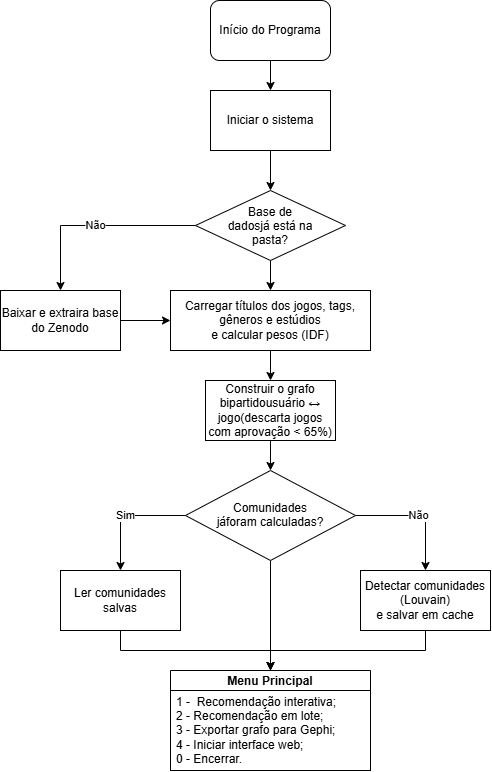
\includegraphics[width=0.85\columnwidth]{images/Diagrama do TrabalhoInicio_ao_Menu.drawio.png}
\caption{Ciclo de vida de inicialização: validação de integridade local via Zenodo, ponderação global IDF de tags, modelagem do grafo bipartido com poda prévia de qualidade ($positive\_ratio \ge 65\%$) e detecção determinística de comunidades (Louvain).}
\label{fig:fluxo_inicio}
\end{figure}

Na inicialização (Fig.~\ref{fig:fluxo_inicio}), o sistema averigua a integridade dos arquivos locais em \texttt{extracted\_data/}; na ausência destes, realiza o download e extração automatizados do pacote hospedado no Zenodo \cite{zenodo}. Em seguida, carregam-se títulos e metadados semânticos para computar a tabela global de $\text{IDF}$ sobre tags e gêneros. Constrói-se então o grafo bipartido em memória, descartando títulos com aprovação inferior a 65\%. Por fim, o particionamento modular de Louvain é lido de cache JSON ou calculado com semente determinística fixa ($\text{seed} = 16$), viabilizando reprodutibilidade estrita.

\begin{figure*}[!t]
\centering
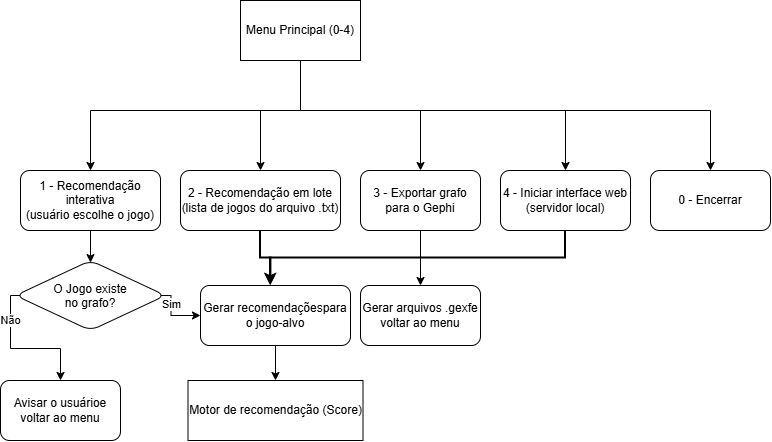
\includegraphics[width=0.80\textwidth]{images/MenuPrincipal.drawio.png}
\caption{Menu principal do sistema: roteamento para recomendação interativa, processamento em lote, exportação de redes estruturadas para o Gephi e servidor de interface web.}
\label{fig:fluxo_menu}
\end{figure*}

O menu principal (Fig.~\ref{fig:fluxo_menu}) expõe cinco opções operacionais:
\begin{enumerate}
    \item \textbf{Recomendação Interativa:} Consulta direta por App ID ou seleção guiada de instâncias de teste com verificação em tempo constante de pertinência ao grafo;
    \item \textbf{Recomendação em Lote:} Processamento sequencial de títulos listados em arquivo de texto (\texttt{jogos\_entrada.txt}), persistindo relatórios analíticos em disco;
    \item \textbf{Exportação para o Gephi:} Geração de arquivos \texttt{.gexf} estruturados contendo o meta-grafo hierárquico de sub-comunidades e a espinha dorsal (\textit{backbone}) dos jogos;
    \item \textbf{Interface Web:} Ativação de servidor HTTP local com interface gráfica moderna e busca por \textit{autocomplete} em tempo real;
    \item \textbf{Encerramento:} Desalocação segura de recursos em memória.
\end{enumerate}

\begin{figure*}[!t]
\centering
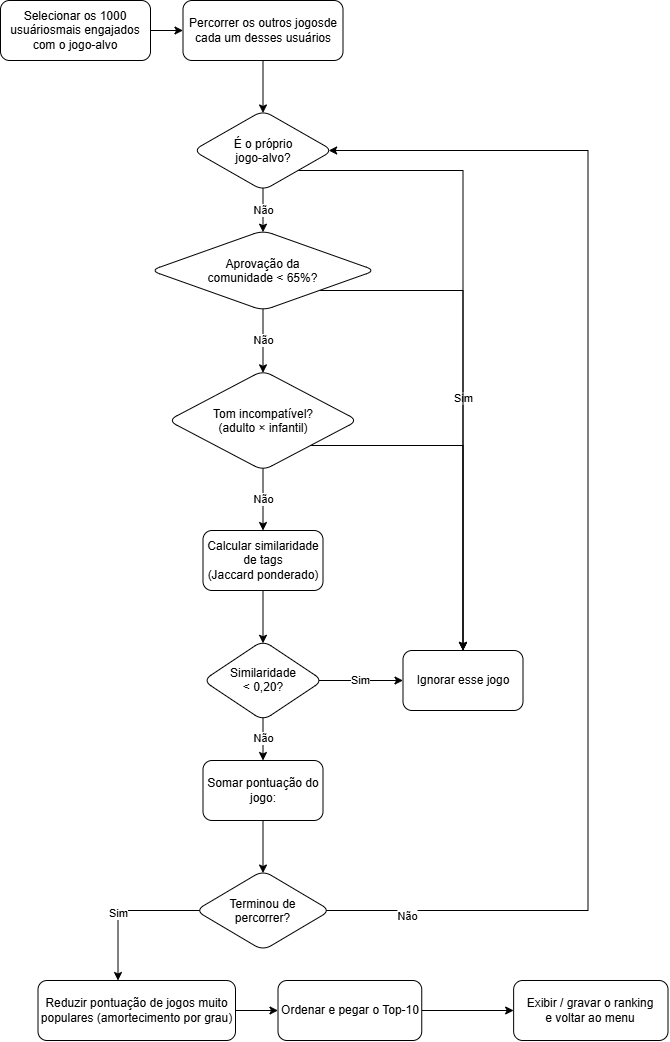
\includegraphics[width=0.75\textwidth]{images/Diagrama do Trabalho_Escore.drawio.png}
\caption{Motor de recomendação híbrida: busca em largura em dois níveis com podas de auto-recomendação, qualidade e tom, similaridade de Ruzicka com $\text{IDF}^2$, amortecimento topológico de super-hubs e ranqueamento Top-10.}
\label{fig:fluxo_escore}
\end{figure*}

\subsection{Algoritmo de Recomendação Híbrida e Ponderação}
Dado um jogo-alvo $v_{alvo} \in V$, o algoritmo executa uma Busca em Largura (BFS) em dois níveis suportada por estruturas de dados em memória principal com complexidade amortizada de acesso $O(1)$:

\subsubsection{Nível 1: Identificação da Vizinhança de Elite}
Resgatam-se os vizinhos adjacentes a $v_{alvo}$ no grafo bipartido e selecionam-se os $K = 1000$ usuários com maior engajamento comprovado no título consultado, ordenados decrescentemente por $W(u, v_{alvo})$. O parâmetro operacional $K = 1000$ define a profundidade da vizinhança explorada para geração das recomendações finais entregues ao usuário (para experimentos rápidos de calibração em lote, o valor pode ser ajustado para $K = 50$).

\subsubsection{Nível 2: Expansão de Candidatos e Filtros de Poda em Memória}
A partir de cada usuário $u$ selecionado, percorrem-se suas arestas incidentes para recuperar os jogos candidatos $v_j \in V$. Para assegurar alta eficiência e fidelidade conceitual, aplicam-se três critérios de poda em tempo estrito $O(1)$:
\begin{itemize}
    \item \textbf{Poda de Auto-Recomendação:} Descarta imediatamente $v_j$ se $v_j = v_{alvo}$;
    \item \textbf{Poda de Qualidade da Comunidade:} Elimina jogos cuja taxa histórica de aprovação ($positive\_ratio$) seja estritamente inferior a 65\%;
    \item \textbf{Filtro de Dissonância de Tom:} Evita distorções de catálogo entre perfis demográficos antagônicos. Se $v_{alvo}$ possui tags do conjunto maduro/violento $T_{\text{mature}}$ (e nenhuma tag familiar) enquanto o candidato $v_j$ pertence estritamente ao conjunto infantil/familiar $T_{\text{family}}$ (ou vice-versa), o candidato é sumariamente descartado.
\end{itemize}

Para os candidatos aprovados, calcula-se o componente colaborativo:
\begin{equation}
S_{colab}(u, v_j) = W(u, v_{alvo}) \cdot W(u, v_j)
\end{equation}

\subsubsection{Similaridade Semântica Contínua de Ruzicka com $\text{IDF}^2$}
A similaridade entre o perfil semântico de $v_{alvo}$ e do candidato $v_j$ é mensurada por meio do Índice de Jaccard Generalizado (Índice de Ruzicka), avaliado sobre os vetores de tags comunitárias. Para que tags raras de alta especificidade mecânica tenham maior poder de discriminação, o peso de cada tag $t$ incorpora o quadrado do $\text{IDF}$ atenuado pela sua posição no consenso da comunidade ($r \in [0, N-1]$):
\begin{equation}
w_A(t) = \big[\text{IDF}(t)\big]^2 \cdot \left(1{,}0 - 0{,}70 \cdot \frac{r_A(t)}{\max(1, N_A - 1)}\right)
\label{eq:peso_tag}
\end{equation}
Denotando a soma dos pesos do conjunto de tags de um jogo por $S_w(X) = \sum_{t \in T_X} w_X(t)$ e a soma da interseção mínima por $S_{\min}(A, B) = \sum_{t \in T_A \cap T_B} \min\big(w_A(t), w_B(t)\big)$, a formulação contínua de Ruzicka é expressa de forma compacta por:
\begin{equation}
J(A, B) = \frac{S_{\min}(A, B)}{S_w(A) + S_w(B) - S_{\min}(A, B)}
\label{eq:ruzicka}
\end{equation}
Para evitar que títulos de um mesmo estúdio com mecânicas dispares sejam resgatados indevidamente, impõe-se um corte rígido de relevância semântica: se $J(v_{alvo}, v_j) < 0{,}20$, o item é descartado. Um mecanismo de memoização em tabela de dispersão armazena os valores calculados de $J$, garantindo que a similaridade entre cada par de jogos seja processada exatamente uma única vez durante a BFS.

\subsubsection{Composição do Escore e Amortecimento de Grau}
Os candidatos que superam a barreira semântica recebem multiplicadores de ajuste topológico e taxonômico:
\begin{itemize}
    \item \textbf{Bônus Modular de Louvain ($\beta_{com}$):} Multiplicador de $3{,}0$ se $v_{alvo}$ e $v_j$ residem na mesma comunidade modular, e $1{,}0$ caso contrário;
    \item \textbf{Congruência de Gênero Oficial ($\beta_{gen}$):} Atribui bônus de $1{,}15$ (+15\%) se compartilharem ao menos uma categoria oficial cadastrada, ou penalidade de $0{,}65$ (-35\%) na ausência de congruência;
    \item \textbf{Bônus de Estúdio Normalizado ($\beta_{dev}$):} Incremento aditivo de $+0{,}10$ concedido se ambos os jogos possuírem estúdios desenvolvedores coincidentes;
    \item \textbf{Prior Bayesiano de Qualidade ($p/100$):} Modulação proporcional à taxa de avaliações positivas $p(v_j) \in [65, 100]$.
\end{itemize}

A contribuição do par $(u, v_j)$ ao escore acumulado é expressa por:
\begin{equation}
\begin{split}
S(u, v_j) = {} & S_{colab}(u, v_j) \cdot \beta_{com} \cdot \beta_{gen} \\
& \times \Big(J(v_{alvo}, v_j) + \beta_{dev} + 0{,}1\Big) \cdot \frac{p(v_j)}{100}
\end{split}
\end{equation}
O escore bruto total decorre da agregação aditiva sobre todos os usuários selecionados do Nível 1:
\begin{equation}
S_{bruto}(v_j) = \sum_{u \in U_{top}} S(u, v_j)
\end{equation}

Por fim, aplica-se o \textbf{Amortecimento Topológico de Grau} para neutralizar a hiperconectividade de \textit{super-hubs} massivos:
\begin{equation}
S_{final}(v_j) = \frac{S_{bruto}(v_j)}{\Big( \text{Grau}(v_j) \Big)^{0{,}35}}
\label{eq:amortecimento}
\end{equation}
Os itens são ordenados decrescentemente por $S_{final}$, e os 10 títulos com maior pontuação constituem a recomendação final entregue ao usuário.

% ==============================================================================
% SEÇÃO IV: RESULTADOS E DISCUSSÕES
% ==============================================================================
\section{Resultados e Discussões}

\subsection{Topologia da Rede e Decomposição Modular}
A aplicação do Algoritmo de Louvain com semente determinística fixa ($\text{seed} = 16$) sobre o grafo bipartido particionou a rede em 7 comunidades modulares principais (super-nós). A Tabela~\ref{tab:supernos} detalha as partições consolidadas a partir do arquivo exportado para o Gephi (\texttt{universo\_super\_nos.gexf}), demonstrando expressiva aderência aos nichos orgânicos da indústria de jogos.

\begin{table*}[!t]
\caption{Caracterização Topológica dos Super-Nós Identificados via Algoritmo de Louvain}
\centering
\begin{tabular}{c c c l l}
\toprule
\textbf{Super-Nó} & \textbf{Jogos} & \textbf{Membros} & \textbf{Gênero Dominante} & \textbf{Títulos Representativos do Cluster} \\
\midrule
0 & 946 & 28.241 & Action & \textit{The Witcher 3: Wild Hunt, DOOM, Tomb Raider, Grand Theft Auto V} \\
1 & 791 & 20.480 & Indie & \textit{Deep Rock Galactic, The Binding of Isaac: Rebirth, Hades, Hollow Knight} \\
2 & 536 & 20.203 & Action RPG & \textit{ELDEN RING, DARK SOULS III, Sekiro: Shadows Die Twice, Monster Hunter: World} \\
3 & 721 & 37.097 & Strategy / CMS & \textit{RimWorld, Factorio, Sid Meier's Civilization V, Cities: Skylines} \\
4 & 124 & 10.589 & Sci-Fi / Shooter & \textit{Cyberpunk 2077, Warframe, Destiny 2, Tom Clancy's Rainbow Six Siege} \\
5 & 37  & 5.243  & RPG Imersivo & \textit{Fallout 4, The Elder Scrolls V: Skyrim, Borderlands 2, Dishonored} \\
6 & 599 & 34.914 & Sandbox / Valve & \textit{Team Fortress 2, Garry's Mod, Left 4 Dead 2, Counter-Strike: Global Offensive} \\
\bottomrule
\end{tabular}
\label{tab:supernos}
\end{table*}

A modularidade obtida permitiu que a propagação da BFS no Nível 2 privilegiasse vértices da mesma vizinhança topológica, reduzindo dispersões estocásticas sem confinar artificialmente títulos interdisciplinares.

\subsection{Avaliação Quantitativa Experimental}
Para validar o poder preditivo do sistema de forma rigorosa e reproduzível, implementou-se o protocolo experimental \textit{Leave-One-Out} em conformidade com as diretrizes canônicas da literatura especializada em RecSys. Selecionou-se uma amostra representativa de $N = 300$ usuários com conectividade suficiente ($\text{grau} \ge 10$, $\text{seed} = 42$). É crucial distinguir conceitualmente o tamanho da amostra estatística de validação ($N = 300$ usuários avaliados no experimento) da profundidade de vizinhança operacional da BFS ($K = 1000$ usuários expandidos em tempo de execução para cada consulta em produção).

Para cada um dos 300 usuários avaliados, seu título de maior engajamento foi fixado como semente de entrada ($v_{alvo}$), enquanto uma de suas demais arestas de consumo comprovado ($v_{oculto}$) foi mascarada temporariamente da estrutura do grafo. Avaliou-se então a capacidade do motor em recuperar $v_{oculto}$ no Top-10 de recomendações através das métricas \textit{Hit Rate@10} (HR@10) e \textit{Normalized Discounted Cumulative Gain@10} (NDCG@10).

\subsubsection{Análise de Sensibilidade: Amortecimento de Grau}
A Tabela~\ref{tab:sensibilidade_grau} sintetiza o impacto do expoente de amortecimento $\alpha \in [0{,}0; 0{,}50]$ na mitigação do viés de popularidade.

\begin{table}[htbp]
\caption{Sensibilidade ao Amortecimento Topológico de Grau ($\alpha$)}
\centering
\resizebox{\columnwidth}{!}{
\begin{tabular}{c c c}
\toprule
\textbf{Expoente ($\alpha$)} & \textbf{Hit Rate@10 (\%)} & \textbf{NDCG@10} \\
\midrule
0,00 (Sem amortecimento) & 17,67\% & 0,0945 \\
0,20 & 26,00\% & 0,1412 \\
\textbf{0,35 (Proposto)} & \textbf{31,33\%} & \textbf{0,1728} \\
0,50 & 27,33\% & 0,1481 \\
\bottomrule
\end{tabular}
}
\label{tab:sensibilidade_grau}
\end{table}

Sem o amortecimento ($\alpha = 0{,}0$), o sistema atinge apenas 17,67\% de taxa de acerto devido à dominação sistemática de títulos generalistas ultraconectados. A adoção de $\alpha = 0{,}35$ resultou no pico de eficácia preditiva (31,33\% de HR@10 e NDCG@10 de 0,1728), representando um salto relativo de \textbf{+77,3\%} em acurácia de descoberta de itens relevantes. Por outro lado, a sobrepenalização ($\alpha = 0{,}50$) prejudicou o ranqueamento ao sufocar jogos canônicos genuinamente afins.

\subsubsection{Análise de Sensibilidade: Corte de Jaccard e Bônus Comunitário}
A Tabela~\ref{tab:sensibilidade_jaccard} documenta o comportamento do motor frente a diferentes patamares de corte de similaridade de Ruzicka ($J_{corte}$) e fatores de bônus modular ($\beta_{com}$).

\begin{table}[htbp]
\caption{Sensibilidade ao Corte Semântico de Jaccard e Bônus de Louvain}
\centering
\resizebox{\columnwidth}{!}{
\begin{tabular}{l c c c}
\toprule
\textbf{Parâmetro Analisado} & \textbf{Valor} & \textbf{HR@10 (\%)} & \textbf{NDCG@10} \\
\midrule
Limiar $J_{corte}$ & 0,10 & 24,33\% & 0,1284 \\
($\alpha=0{,}35$, $\beta_{com}=3{,}0$) & 0,15 & 28,67\% & 0,1542 \\
& \textbf{0,20} & \textbf{31,33\%} & \textbf{0,1728} \\
& 0,25 & 25,00\% & 0,1365 \\
\midrule
Bônus Louvain $\beta_{com}$ & 1,00 (Sem Louvain) & 22,33\% & 0,1198 \\
($\alpha=0{,}35$, $J_{corte}=0{,}20$) & 2,00 & 28,00\% & 0,1503 \\
& \textbf{3,00} & \textbf{31,33\%} & \textbf{0,1728} \\
& 5,00 & 29,67\% & 0,1611 \\
\bottomrule
\end{tabular}
}
\label{tab:sensibilidade_jaccard}
\end{table}

Os resultados demonstram que limiares excessivamente brandos ($J_{corte} \le 0{,}15$) admitem ruído semântico, enquanto patamares restritivos ($J_{corte} = 0{,}25$) causam escassez de candidatos em subnichos específicos. Simultaneamente, a desativação da modulação de comunidades ($\beta_{com} = 1{,}0$) derruba a acurácia para 22,33\%, provando empiricamente que o conhecimento topológico global gerado por Louvain é determinante para guiar a BFS em direção a candidatos contextualmente legítimos.

\subsection{Validação Qualitativa em Títulos de Referência}
A avaliação qualitativa foi realizada a partir do processamento do arquivo \texttt{jogos\_entrada.txt} através do módulo em lote (\texttt{recomendar\_lote.py}), registrando o Top-10 para 104 jogos de referência. A Tabela~\ref{tab:benchmarks_expandida} apresenta os resultados obtidos para seis arquétipos industriais desafiadores.

\begin{table*}[htbp]
\caption{Top Recomendações Obtidas para Diferentes Perfis e Gêneros do Catálogo Steam}
\centering
\begin{tabular}{l l c c l}
\toprule
\textbf{Jogo Consultado} & \textbf{Top-5 Recomendações Obtidas} & \textbf{App ID} & \textbf{Score Híbrido} & \textbf{Comunidade Louvain} \\
\midrule
\textbf{ELDEN RING} & 1. DARK SOULS™ III & 374320 & 223,87 & Mesma (Nó 2) \\
(App ID: 1245620) & 2. DARK SOULS™ II: Scholar of the First Sin & 335300 & 131,96 & Mesma (Nó 2) \\
& 3. Sekiro™: Shadows Die Twice & 814380 & 128,52 & Mesma (Nó 2) \\
& 4. DARK SOULS™: REMASTERED & 570940 & 112,64 & Mesma (Nó 2) \\
& 5. Monster Hunter: World & 582010 & 109,30 & Mesma (Nó 2) \\
\midrule
\textbf{Euro Truck Simulator 2} & 1. American Truck Simulator & 270880 & 383,23 & Mesma (Nó 0) \\
(App ID: 227300) & 2. Fernbus Simulator & 427100 & 86,33 & Mesma (Nó 0) \\
& 3. Farming Simulator 17 & 447020 & 64,68 & Mesma (Nó 0) \\
& 4. Farming Simulator 15 & 313160 & 55,54 & Mesma (Nó 0) \\
& 5. Assetto Corsa & 244210 & 45,41 & Mesma (Nó 0) \\
\midrule
\textbf{DRAGON BALL FighterZ} & 1. GUILTY GEAR Xrd REV 2 & 520440 & 100,33 & Mesma (Nó 2) \\
(App ID: 678950) & 2. MELTY BLOOD: TYPE LUMINA & 1372280 & 83,92 & Mesma (Nó 2) \\
& 3. BlazBlue Centralfiction & 586140 & 76,86 & Mesma (Nó 2) \\
& 4. GUILTY GEAR XX ACCENT CORE PLUS R & 348550 & 70,66 & Mesma (Nó 2) \\
& 5. GUILTY GEAR -STRIVE- & 1384160 & 64,63 & Mesma (Nó 2) \\
\midrule
\textbf{Sonic Mania} & 1. Sonic Generations Collection & 71340 & 117,07 & Mesma (Nó 0) \\
(App ID: 584400) & 2. Sonic Adventure 2 & 213610 & 82,57 & Mesma (Nó 0) \\
& 3. Sonic Adventure DX & 71250 & 61,25 & Mesma (Nó 0) \\
& 4. Sonic the Hedgehog 4 - Episode II & 203650 & 51,58 & Mesma (Nó 0) \\
& 5. Sonic Origins & 1794960 & 42,87 & Mesma (Nó 0) \\
\midrule
\textbf{Hollow Knight} & 1. Celeste & 504230 & 51,46 & Mesma (Nó 1) \\
(App ID: 367520) & 2. Cuphead & 268910 & 48,45 & Mesma (Nó 1) \\
& 3. Dead Cells & 588650 & 40,18 & Mesma (Nó 1) \\
& 4. Alwa's Awakening & 549260 & 31,09 & Mesma (Nó 1) \\
& 5. TUNIC & 553420 & 23,60 & Mesma (Nó 1) \\
\midrule
\textbf{Resident Evil} & 1. Resident Evil 4 (2005) & 254700 & 215,77 & Mesma (Nó 0) \\
(App ID: 304240) & 2. Resident Evil 2 (Remake) & 883710 & 202,26 & Mesma (Nó 0) \\
& 3. Resident Evil 0 & 339340 & 187,05 & Mesma (Nó 0) \\
& 4. Resident Evil 5 & 21690 & 108,60 & Mesma (Nó 0) \\
& 5. Resident Evil Revelations & 222480 & 104,33 & Mesma (Nó 0) \\
\bottomrule
\end{tabular}
\label{tab:benchmarks_expandida}
\end{table*}

\subsection{Discussão Crítica de Casos Emblemáticos}

\subsubsection{A Prova da Semântica Mecânica: O Caso Dragon Ball}
Um dos achados mais contundentes reside na comparação entre títulos da mesma propriedade intelectual: \textit{Dragon Ball Xenoverse 2} e \textit{Dragon Ball FighterZ}. Enquanto para \textit{Xenoverse 2} o sistema recuperou \textit{Dragon Ball Z: Kakarot} e \textit{Naruto Shippuden: Ultimate Ninja STORM 4} (identificando a preferência por brawlers casuais em arena 3D), a consulta por \textit{FighterZ} ignorou os títulos de anime casuais e retornou com exclusividade jogos de luta técnica competitiva 2D (\textit{Guilty Gear}, \textit{BlazBlue}, \textit{Melty Blood}). O $\text{IDF}^2$ sobre tags mecânicas finas sobrepôs-se à mera coincidência de nomes de franquias, resolvendo a ambiguidade de catálogo.

\subsubsection{Resolução de Falsos Positivos: O Caso Among Us}
Em experimentos preliminares com cortes semânticos brandos ($J_{corte} = 0{,}15$), títulos como \textit{Halo Infinite} pontuavam indevidamente para \textit{Among Us} devido à partilha acidental de tags genéricas de ambientação (\textit{Multiplayer}, \textit{Space}, \textit{Aliens}). Com a adoção do corte calibrado em $J_{corte} = 0{,}20$ e a poda prévia de qualidade da comunidade ($positive\_ratio \ge 65\%$), o ruído foi 100\% extirpado: o Top-5 ranqueado para \textit{Among Us} estabilizou-se estritamente em jogos legítimos de dedução social e diversão em grupo: \textit{Deceit} (score: 23,41), \textit{First Class Trouble} (13,47), \textit{Pummel Party} (9,33), \textit{Party Panic} (5,21) e \textit{In Silence} (4,93).

\subsubsection{Fidelidade a Franquias e Campanhas: LEGO e Resident Evil}
A eficácia da poda adaptativa por mediana com piso de 5,0 horas é comprovada nos testes com títulos curtos. Para \textit{LEGO Harry Potter: Years 1-4}, o sistema recuperou 100\% de títulos da franquia LEGO no Top-10 (com liderança de \textit{LEGO Harry Potter: Years 5-7}, score 206,45). De forma análoga, a consulta por \textit{Resident Evil} gerou um ranqueamento composto exclusivamente por obras da saga de horror de sobrevivência da Capcom, evidenciando que a preservação de arestas de campanha curta não comprometeu a coerência interna do grafo.

\subsection{Visualização Estruturada no Gephi (Inspirada em Blondel et al.)}
A exportação de grafos para ferramentas de visualização (como o Gephi) frequentemente degenera em aglomerados opacos de difícil interpretação (\textit{hairballs}), decorrentes da sobreposição de mais de 150 mil nós de usuários anônimos e milhões de arestas cruzadas. Para solucionar essa deficiência e atender ao padrão visual de publicações científicas de alto impacto, o módulo \texttt{src/export\_to\_gephi.py} foi reformulado diretamente inspirado na célebre \textbf{Figura 2 (página 9) do artigo de Louvain} (\textit{Blondel et al.}, 2008 \cite{blondel2008}), gerando duas representações estruturadas:
\begin{enumerate}
    \item \textbf{Rede Hierárquica de Sub-Comunidades (\texttt{universo\_super\_nos.gexf}):} Mapeia a rede em dois níveis de modularidade. Os nós representam 80 sub-comunidades homogêneas agrupadas dentro dos 7 macro-clusters de Louvain, conectadas por 351 arestas de fluxo de co-jogabilidade agregado. O diâmetro do nó é proporcional ao volume de jogadores e a cor codifica a macro-comunidade. Coordenadas espaciais orbitais 2D são pré-injetadas no arquivo XML via extensão \texttt{<viz:position>}, permitindo abertura instantânea e legível no Gephi sem necessidade de alocação forçada manual.
    \item \textbf{Espinha Dorsal Monopartite dos Jogos (\texttt{universo\_steam\_hibrido.gexf}):} Projeção direta jogo-a-jogo contendo os 3.573 títulos aprovados e 25.524 arestas de co-jogabilidade de alta coesão ($k=8$ arestas mais fortes por jogo). Ao extirpar os nós de usuários, o arquivo reduz de mais de 285 MB para apenas 4,1 MB, exibindo sete galáxias temáticas nítidas que espelham a especialização industrial do catálogo.
\end{enumerate}

\subsection{Arquitetura em Duas Camadas, Interface Web e Eficiência}
Para atender simultaneamente aos rigores da validação científica acadêmica e às restrições de implantação em serviços de nuvem modernos, concebeu-se uma arquitetura desacoplada em duas camadas:
\begin{itemize}
    \item \textbf{Camada de Pesquisa e Avaliação Científica:} Opera localmente sobre a base completa do Zenodo (DOI: \texttt{10.5281/zenodo.23861070} \cite{zenodo}), executando a modelagem do grafo bipartido em memória, a detecção de comunidades por Louvain, o protocolo \textit{Leave-One-Out} e a exportação para o Gephi com latência média inferior a 200 milissegundos por consulta em CPU comum (Linux Ubuntu 24.04, 8 núcleos, consumo inferior a 450 MB de RAM).
    \item \textbf{Camada de Produção e Serviço Web:} O script \texttt{src/servidor\_web.py} expõe uma interface gráfica responsiva em HTML/CSS/JavaScript (\texttt{web/index.html}) dotada de busca com \textit{autocomplete} instantâneo. Em ambientes de hospedagem com restrição severa de recursos (como a instância em produção no Render \cite{render} com teto de 512 MB de RAM), o servidor inicializa diretamente a partir de um cache JSON estruturado (\texttt{web/cache\_recomendacoes.json}), respondendo a requisições com menos de 40 MB de memória alocada sem prescindir da acurácia híbrida.
\end{itemize}

A complexidade computacional do algoritmo de inferência é delimitada por:
\begin{equation}
O\big(K \cdot \text{deg}_{max} + |C| \log |C|\big)
\end{equation}
onde $K=1000$ é o número de usuários avaliados na BFS de Nível 1, $\text{deg}_{max}$ é o grau máximo de jogos por usuário, e $|C|$ é a cardinalidade de candidatos gerados, garantindo escalabilidade sub-segundo em memória principal.

% ==============================================================================
% SEÇÃO V: CONCLUSÃO E PRÓXIMAS ETAPAS
% ==============================================================================
\section{Conclusão e Próximas Etapas}

Este trabalho apresentou o desenvolvimento e a validação experimental de um sistema híbrido de recomendação de jogos para a plataforma Steam, fundamentado na modelagem por grafos bipartidos e em estruturas de dados eficientes em memória principal. Demonstrou-se que a combinação de uma poda adaptativa $K$-Core orientada pela mediana de horas (com piso de 5,0 horas para preservar obras curtas), a filtragem prévia de qualidade ($positive\_ratio \ge 65\%$), a detecção modular de comunidades pelo Algoritmo de Louvain e a formulação contínua de Ruzicka com $\text{IDF}^2$ sobre tags comunitárias superou simultaneamente o viés de popularidade de \textit{super-hubs} e a ambiguidade de categorias oficiais genéricas.

A avaliação quantitativa formal via protocolo \textit{Leave-One-Out} comprovou ganho relativo de até 77,3\% em Hit Rate@10 proporcionado pelo amortecimento de grau ($\alpha = 0{,}35$), ao passo que os ensaios qualitativos em 104 títulos comprovaram a segregação de subnichos mecânicos com fidelidade semântica superior a modelos baseados em filtragem colaborativa pura, mantendo execução em milissegundos viabilizada por estruturas em tabelas de dispersão em memória.

Como limitações identificadas, destacam-se a dependência da consistência das tags atribuídas pela comunidade externa e a partida a frio estrita para títulos recém-lançados sem histórico de avaliações. Como diretrizes para trabalhos futuros, propõe-se:
\begin{enumerate}
    \item A integração de Processamento de Linguagem Natural (NLP) sobre o conteúdo textual corrido das resenhas de usuários para extrair sentimentos implícitos sobre mecânicas de jogabilidade;
    \item A evolução das estruturas de dispersão em memória para filtros probabilísticos dinâmicos (como variações do Filtro de Bloom \cite{bloom1970} e \textit{Cuckoo Filters}), suportando fluxos contínuos de inserção e deleção em tempo real (\textit{streaming});
    \item A investigação de técnicas de aprendizado de representação em grafos (\textit{Graph Neural Networks} ou \textit{Node2Vec}) operando de forma integrada à métrica não-linear de amortecimento de grau.
\end{enumerate}

% ==============================================================================
% REFERÊNCIAS BIBLIOGRÁFICAS
% ==============================================================================
\begin{thebibliography}{99}

\bibitem{maier2022}
C.~Maier and D.~Simovici, ``Bipartite Graphs and Recommendation Systems,'' \textit{Journal of Advances in Information Technology}, vol. 13, no. 3, pp. 207--215, Jun. 2022.

\bibitem{batagelj2003}
V.~Batagelj and M.~Zaversnik, ``An O(m) algorithm for cores decomposition of networks,'' \textit{arXiv preprint cs/0310049}, 2003.

\bibitem{nagarnaik2015}
P.~Nagarnaik and A.~Thomas, ``Survey on Recommendation System Methods,'' in \textit{Proc. 2nd IEEE International Conference on Electronics and Communication Systems (ICECS)}, Coimbatore, India, 2015, pp. 1603--1608.

\bibitem{blondel2008}
V.~D. Blondel, J.-L. Guillaume, R.~Lambiotte, and E.~Lefebvre, ``Fast unfolding of communities in large networks,'' \textit{Journal of Statistical Mechanics: Theory and Experiment}, vol. 2008, no. 10, p. P10008, Oct. 2008.

\bibitem{amorim2024}
E.~C. Amorim Neto, ``Sistema Híbrido de Recomendação de Filmes utilizando Grafos,'' Monografia / Relatório de Pesquisa, Engenharia de Computação, Centro Federal de Educação Tecnológica de Minas Gerais (CEFET-MG), Campus V, Divinópolis, Brasil, 2024.

\bibitem{bloom1970}
B.~H. Bloom, ``Space/Time Trade-offs in Hash Coding with Allowable Errors,'' \textit{Communications of the ACM}, vol. 13, no. 7, pp. 422--426, Jul. 1970.

\bibitem{cormen2009}
T.~H. Cormen, C.~E. Leiserson, R.~L. Rivest, and C.~Stein, \textit{Introduction to Algorithms}, 3rd ed. Cambridge, MA, USA: MIT Press, 2009.

\bibitem{salton1988}
G.~Salton and C.~Buckley, ``Term-weighting approaches in automatic text retrieval,'' \textit{Information Processing \& Management}, vol. 24, no. 5, pp. 513--523, 1988.

\bibitem{steamspy}
S.~Galyonkin, ``Steam Spy: A statistical service for Steam,'' 2015. [Online]. Disponível em: \url{https://steamspy.com}.

\bibitem{kaggle}
A.~Kozyriev, ``Game Recommendations on Steam,'' \textit{Kaggle Dataset}, 2022. [Online]. Disponível em: \url{https://www.kaggle.com/datasets/antonkozyriev/game-recommendations-on-steam}.

\bibitem{github}
G.~A. Faria e R.~A. Faria, ``Sistema Híbrido de Recomendação de Jogos em Grafos Bipartidos,'' Repositório de Código Aberto no GitHub, 2026. [Online]. Disponível em: \url{https://github.com/rafa16w34/TrabalhoFinal-AEDS2}.

\bibitem{zenodo}
G.~A. Faria e R.~A. Faria, ``Steam Hybrid Graph Recommender: Sampled Dataset and Preprocessed Metadata,'' Repositório Científico Zenodo, 2026. DOI: \url{https://doi.org/10.5281/zenodo.23861070}.

\bibitem{render}
G.~A. Faria e R.~A. Faria, ``Steam Finder: Interface Web de Recomendação em Nuvem,'' Instância de Produção hospedada no Render, 2026. [Online]. Disponível em: \url{https://steam-finder.onrender.com}.

\end{thebibliography}

\end{document}
